\documentclass[aspectratio=169,xcolor=table]{beamer}
%aspcetratio >> 1610 169 149 54 43 32
%The themes:
%\usetheme[style=classic]{mharvellous}
%\usetheme[style=dark]{mharvellous}
%\usetheme[style=mracula]{mharvellous}
\usetheme[style=default]{mharvellous}
%*--------------------------------------------------
%\usepackage{helvet}
%*--------------------------------------------------
\usepackage{bibunits}  
%\setbeamertemplate{bibliography item}{[\theenumiv]}
\setbeamertemplate{bibliography item}{\insertbiblabel}
\defaultbibliography{bibliography}
%\defaultbibliographystyle{IEEEtran}
%\defaultbibliographystyle{amsalpha}
\defaultbibliographystyle{abntex2-alf}
%\bibliography{bibliography}
%\usepackage[backend=biber,style=alphabetic,citestyle=authoryear]{biblatex}
% \addbibresource{bibliography.bib}
%\usepackage{natbib}
\usepackage{bibentry}
%*--------------------------------------------------
\usepackage{lipsum}
\usepackage{epigraph}
\usepackage{graphicx}
\usepackage{multirow}
%\usepackage{enumitem}
\usepackage{array}
%\usepackage{multimedia}
\usepackage{media9}
%\usepackage{pdfpc-movie}
\usepackage{circledsteps}
\usepackage{listings}
\usepackage[normalem]{ulem}
%\usepackage{Sweave}
%\usepackage{xkeyval}
%\usepackage{palatino}
%\usepackage{pgfpages}
\usepackage{float}
%*--------------------------------------------------
\usepackage[timeinterval=1]{tdclock}
%\usepackage[font=Times,timeinterval=1, timeduration=200,resetatpages=all]{tdclock}
%\usepackage[font=Times,timeinterval=10, timeduration=2.0, timedeath=0, fillcolorwarningsecond=white!60!yellow,timewarningfirst=50,timewarningsecond=80,resetatpages=2]{tdclock}
%*--------------------------------------------------
\usepackage{url}
\usepackage{tabularx,booktabs}
\usepackage{threeparttable}
\usepackage[absolute, overlay]{textpos}
%*--------------------------------------------------
\usepackage{framed, color}
\usepackage[tikz]{bclogo}
\usepackage{spot}
\setspotlightcolor{red!50}
% %\setspotlightstyle{star, fill=red!50}
% %\setspotlightstyle{star points=7}
\usepackage{color,soul}
%\usepackage{xcolor}
\usepackage{tcolorbox}
\usepackage{xcolor}
\usepackage[export]{adjustbox}
\usepackage{verbatim}
\usetikzlibrary{trees,shapes,arrows}
\usepackage{fancyvrb}
\usepackage{float}
%*--------------------------------------------------
\usepackage{amsmath}
\usepackage{xfrac}
\usepackage{units}
\usepackage{ulem}
%*-------------------------------------------------------------------------------
%\newcolumntype{C}[1]{>{\centering\arraybackslash}m{#1}}
\newcolumntype{L}[1]{>{\raggedright\let\newline\\\arraybackslash\hspace{0pt}}m{#1}}
\newcolumntype{C}[1]{>{\centering\let\newline\\\arraybackslash\hspace{0pt}}m{#1}}
\newcolumntype{R}[1]{>{\raggedleft\let\newline\\\arraybackslash\hspace{0pt}}m{#1}}
%*-------------------------------------------------------------------------------
%\pgfpagesuselayout{2 on 1}[a4paper,border shrink=5mm]
%\setbeamertemplate{note page}[plain]
%\setbeameroption{show notes on second screen=bottom}
%*-------------------------------------------------------------------------------
\setbeameroption{hide notes}
%\setbeameroption{show only notes}
%\setbeameroption{show notes on second screen=right}
\setbeamertemplate{note page}{\pagecolor{yellow!5}\insertnote}
%*-------------------------------------------------------------------------------

%*-------------------------------------------------------------------------------
\title              {JAX Manipulator}
\subtitle           {An Inverse and Forward Kinematic Challenge}
\author             {M. Zarth Seixas \and M. Anselmo da Silva}
\email              {mateus.seixas@fbter.org.br \and matheus.anselmo@fbter.org.br}
\advisor            {Orientador: Marco A. dos Reis}
\institute          {Robótica e Sistemas Autônomos, Senai Cimatec}
\date               {2022 March}
% \ulogo        		{Template/logosenaicimatecnegativo}
% \ulogof             {Template/logosenaicimatec2020}
% \ulogoo        		{Template/rosa-logo}
% \ulistelement    	{Template/bullet-white}

%*-------------------------------------------------------------------------------
\graphicspath{{Source/pictures/}}
%*-------------------------------------------------------------------------------
\totalNoSlidesDisabled % To turn off the total number of slides in the footer. Comment this if you want the total number of slides in the footer
%*-------------------------------------------------------------------------------
\begin{document}
%*----------- COVER -------------------------------------------------------------
 \begin{frame}[t,plain]
%*----------- sound--------------------------------
    \includemedia[
        %width=1ex,
        %height=1ex,
        %activate=pageopen, 
        activate=onclick,
        deactivate=onclick,
        %passcontext,
        transparent,
        addresource=./Source/sounds/hip-hop.mp3,
        flashvars={
                    source=./Source/sounds/hip-hop.mp3
                    %&autoPlay=true
                    &autoRewind=true
                    &Play=2s
                    &repeat=always
                    %&Loop=true
        }
    ]
    {}{VPlayer.swf}
%*----------- start-page--------------------------
    \titlepage
    %*----------- notes-------------------------------
    \note[item]{Notes can help you to remember important information. Turn on the notes option.}
\end{frame}
%-
%*----------- SECTIONS ----------------------------------------------------------
%*----------- SLIDE -------------------------------------------------------------
\begin{frame}[t]{Introdução} 
    \transdissolve[duration=0.5]
   
    Linha de pesquisa focada em estudos e desenvolvimentos em \textbf{robótica submarina}, aspectos de dinâmica computacional, aplicações de funções básicas de robótica e desenvolvimento de tecnologias de busca e análise deste campo.

   
    %\newline
        \begin{columns}[t]
            
            \column{0.33\linewidth}
            \begin{center}
            \begin{figure}
                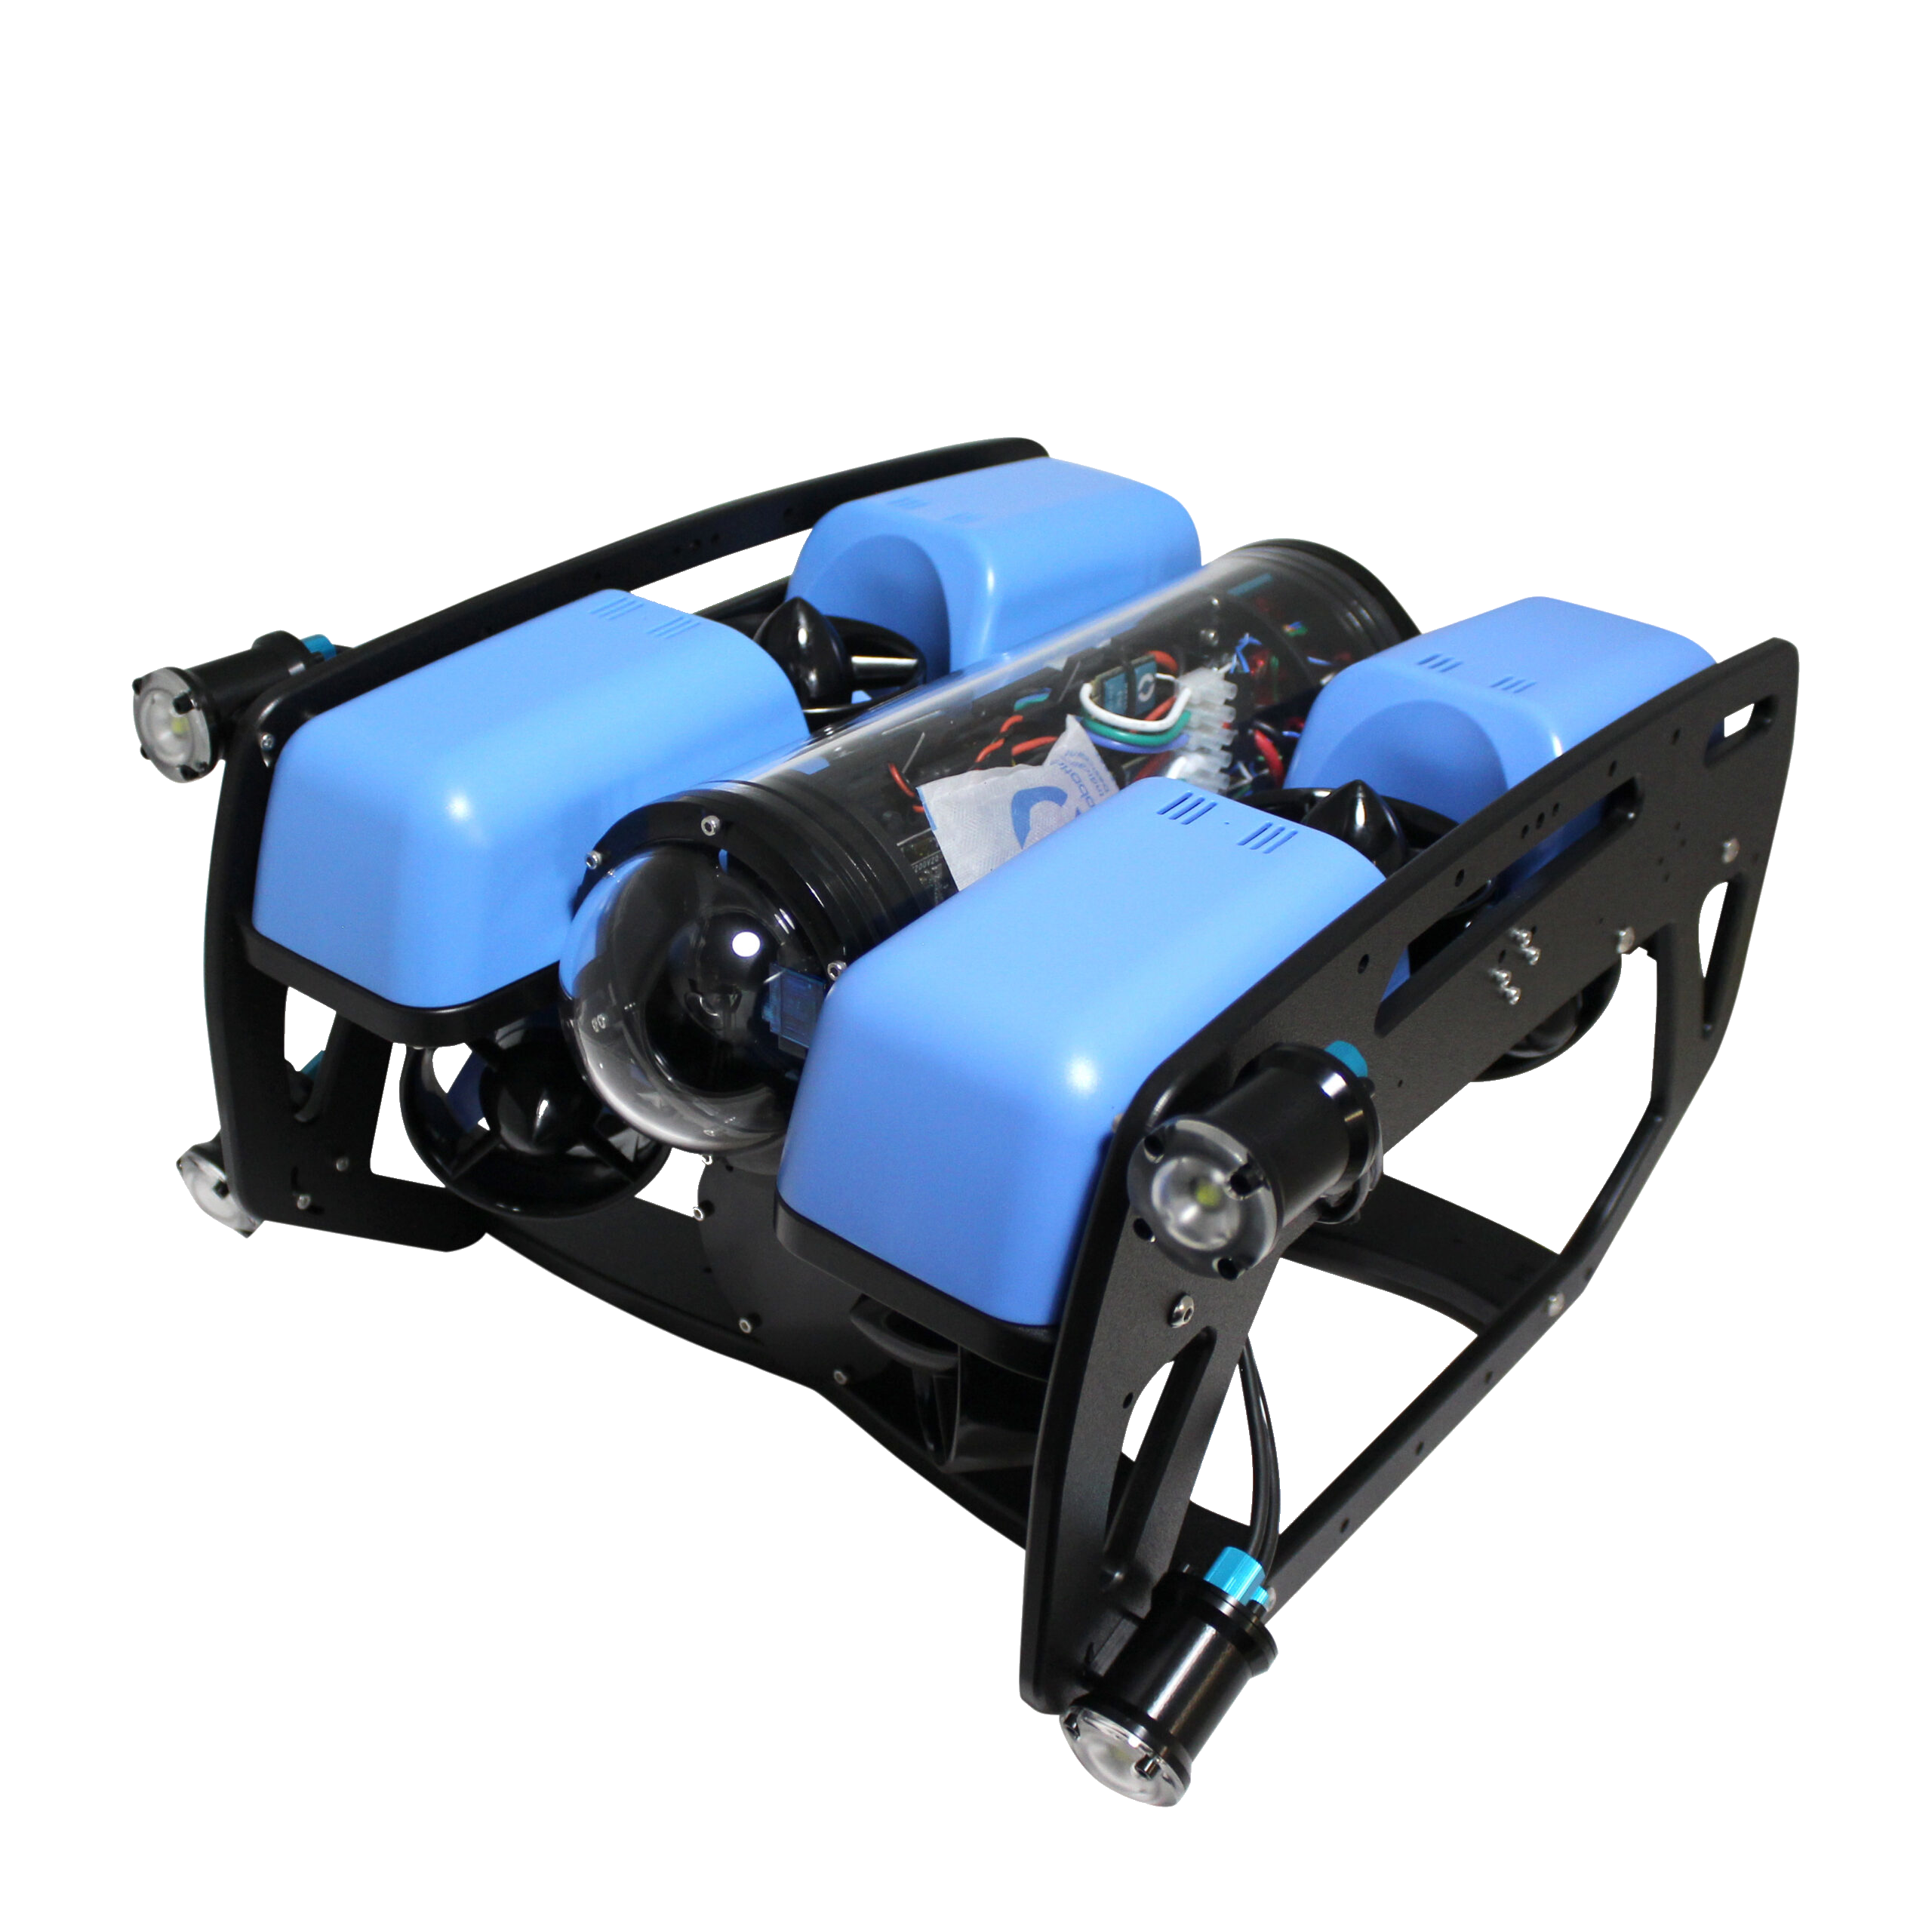
\includegraphics[width=0.8\textwidth]{bluerov.png}
               
               
                  
               
            \end{figure}

            \end{center}
            \column{.33\linewidth}
            \vspace*{0.6cm}
            \begin{center}
          
                \begin{figure}
                    
                    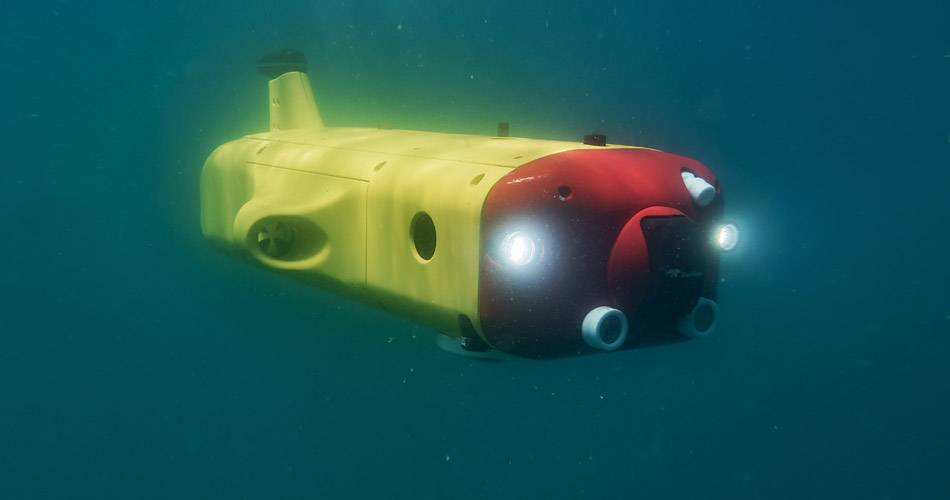
\includegraphics[width=1\textwidth]{flatfish.jpg}
                \end{figure}
            %}
            \end{center}
            
            \column{.33\linewidth}
            \begin{center}
            \vspace*{0.4cm}
            \begin{figure}
                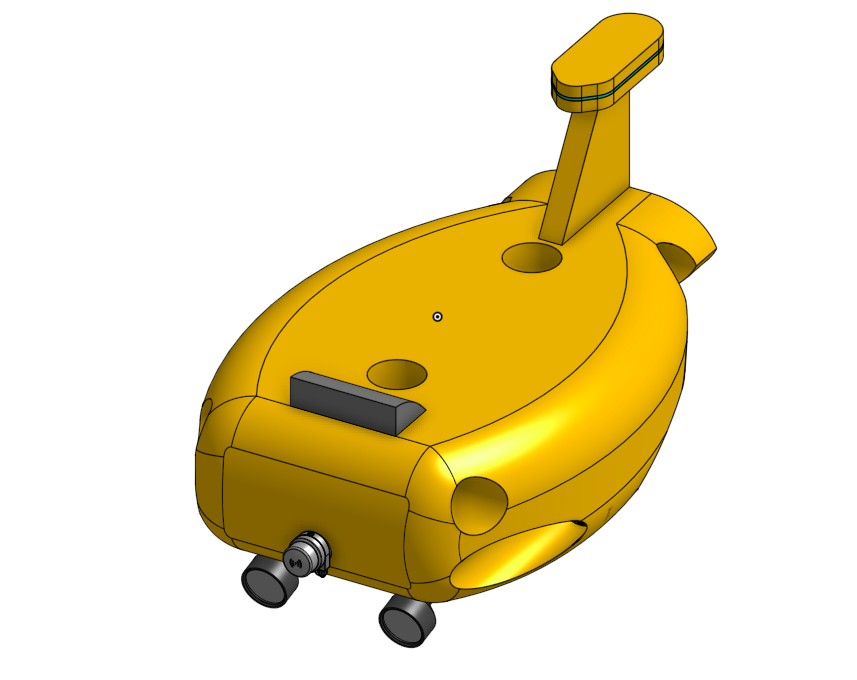
\includegraphics[width=0.8\textwidth]{turbot.png}
            \end{figure}
            \end{center}
        \end{columns}
%*----------- notes
    \note[item]{Notes can help you to remember important information. Turn on the notes option.}
\end{frame}
%-
%*----------- SLIDE -------------------------------------------------------------
\begin{frame}[c]{Objetivos} 
    
    \transdissolve[duration=0.5]
   
    \begin{center}
        \Wider{%
        \begin{shaded}
        \begin{center}
            \vspace*{0.5cm}
            \resizebox{!}{0.5cm}{%
               
                \color{bg} Treinamento de pesquisadores em robótica submarina na água
            }%
        \end{center}
        \end{shaded}
        }%
    \end{center}

\end{frame}


\begin{frame}[t]{Motivação} 
  
  \textbf{AUVs} and \textbf{ROVs} estão um papel importante na exploração de petróleo, gás e de outros recursos. Grandes importantes empresas estão pedindo investimentos nesta área.

  \newline
  \newline
  \newline
  \newline
  \newline
  \\
  \vspace{1.75cm}
  \\
  \begin{center}
  "\textbf{AUV and ROV Market to reach \$7.2 billion by 2026}" \cite{reportlinker}.

\end{center}


\end{frame}




    
   

%%*----------- SLIDE -------------------------------------------------------------
\begin{frame}[t]{Main Tools}
    %\transboxin[duration=1,direction=30]
    In this Field of \textbf{Reasearch} and \textbf{develpoments} there are great tools that can be used.
    \newline
    On the \textbf{reaserch espectrum}

    \\
    \\
    \\

    \\

    \vspace*{1.6cm}

    \begin{columns}[c]
            
        \column{0.25\linewidth}

        \begin{center}
            \begin{figure}
                
\includegraphics[width=0.65\textwidth]{cmap.png}
            \end{figure}
        \end{end}

        \column{0.25\linewidth}

        \begin{center}
            \begin{figure}
                
\includegraphics[width=0.45\textwidth]{mendeley.png}
            \end{figure}
        \end{end}

        \column{0.25\linewidth}

        \begin{center}
            \begin{figure}
                
\includegraphics[width=1\textwidth]{scopus.png}
            \end{figure}
        \end{end}


        \column{0.25\linewidth}
        \begin{center}
            \begin{figure}
                
\includegraphics[width=1\textwidth]{notion1411.png}
        \end{figure}
    \end{end}

    \end{columns}
   
\end{frame}


\begin{frame}[t]{Main Tools}
    %\transboxin[duration=1,direction=30]
   
    \newline
    On the \textbf{develpment espectrum}

    \\
    \\
    \\

    \\

    \vspace*{1.6cm}

    \begin{columns}[c]
            
        \column{0.25\linewidth}

        \begin{center}
            \begin{figure}
                
\includegraphics[width=0.65\textwidth]{cmap.png}
            \end{figure}
        \end{end}

        \column{0.25\linewidth}

        \begin{center}
            \begin{figure}
                
\includegraphics[width=0.45\textwidth]{mendeley.png}
            \end{figure}
        \end{end}

        \column{0.25\linewidth}

        \begin{center}
            \begin{figure}
                
\includegraphics[width=1\textwidth]{scopus.png}
            \end{figure}
        \end{end}


        \column{0.25\linewidth}
        \begin{center}
            \begin{figure}
                
\includegraphics[width=1\textwidth]{notion1411.png}
        \end{figure}
    \end{end}

    \end{columns}
   
\end{frame}
%-
%*----------- SLIDE -------------------------------------------------------------
\begin{frame}[t]{Algumas regras}
    \begin{itemize}
        \item A marcha deverá ser realizada diante de um percurso de 2 metros.
        \item A marcha e a corrida de revezamento deverão serem realizadas numa pista de corrida;
        \item A corrida deverá ser realizada numa pista de 8 metros;
        \item Cada Darwin-OP deverá percorrer 2 metros para realizar o revezamento;
        \item A região de revezamento deverá ser uma área de até 0.4 metros;
        \item O conceito para o revezamento será o de alinhar-se os dois Darwin-OP durante até 15 segundos a uma distância de no máximo 0.2 metros entre ambos, ou seja será considerado passagem de bastão quando os dois Darwin-OP passarem 15 segundos com movimentos sincronizados a uma distância máxima de 0.2 metros dentro da região de revezamento;
        \item A pista de corrida deverá ser considerada analogamente a uma pista real;
        \item A lateral da pista deverá ter lados de 2 metros;
        \item Considerar sempre os critérios de uma corrida de revezamento.
    \end{itemize}
   
    % \begin{columns}[t]
    %     \column{.45\textwidth}
    %         detalhar sistemas em subconjuntos\\
    %         listar possíveis modos de falhas\\
    %         analisar cada modo de falha, juntamente com suas possíveis causas e sintomas
    %     \column{.45\textwidth}
    %         estimar os efeitos de cada modo de falhas\\
    %         estimar a criticidade de cada efeito\\
    %         identificar ações para minimizar falhas
    % \end{columns}
%*----------- notes
    \note[item]{Notes can help you to remember important information. Turn on the notes option.}
\end{frame}
%-
%*----------- SLIDE -------------------------------------------------------------
\begin{frame}[c]{A pista}
    \begin{figure}
        %\includegraphics[width=0.7\textwidth]{pista_corrida}
       
        \roundpic[xshift=0cm,yshift=0cm]{3cm}{7cm}{pista_corrida}
          
        \caption{Formato de um pista de corrida.\cite{agostini2007}}
    \end{figure}
%*----------- notes
    \note[item]{Notes can help you to remember important information. Turn on the notes option.}
\end{frame}
%-
%%*----------- SLIDE -------------------------------------------------------------
\begin{frame}[t]{Arquitetura do Sistema}

    \begin{center}
        \begin{figure}
            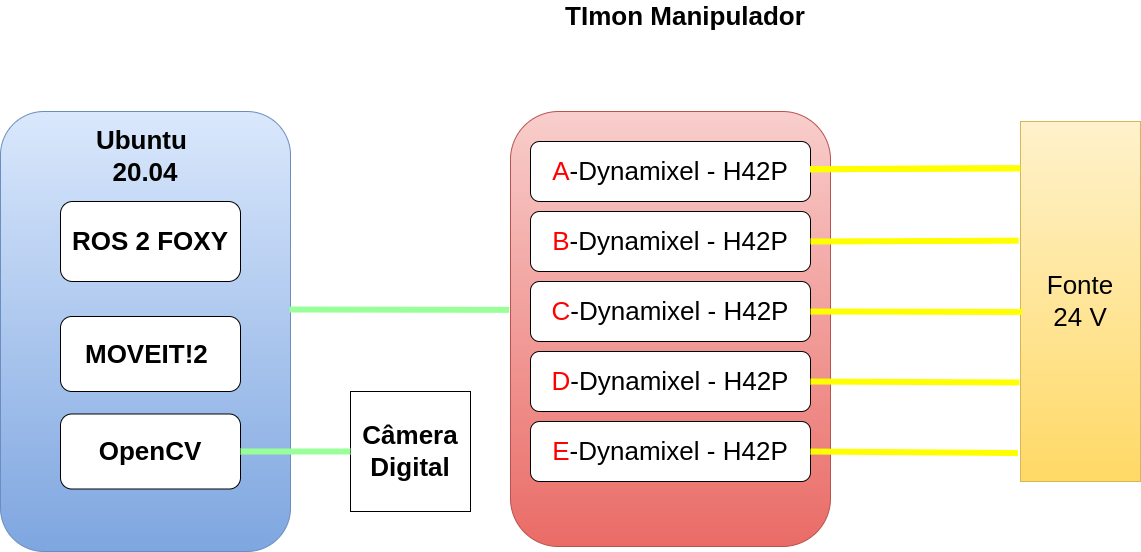
\includegraphics[width=0.9\textwidth]{system_architeture2.png}
            
        \end{figure}
        
    \end{center}
   
\end{frame}


\begin{frame}[t]{Testes dos Motores}
    
    \begin{center}
        \begin{figure}
            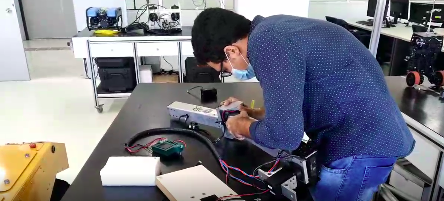
\includegraphics[width=0.75\textwidth]{motor_test.png}
            
        \end{figure}
        
    \end{center}
   
\end{frame}


\begin{frame}[t]{Testes dos Motores}
    
    \begin{center}
        \begin{figure}
            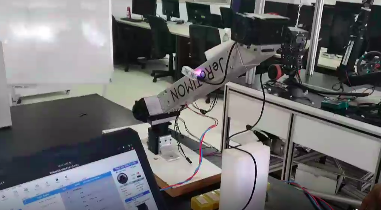
\includegraphics[width=0.75\textwidth]{testmotor_2.png}
            
        \end{figure}
        
    \end{center}
   
\end{frame}



\begin{frame}[t]{Atividades em Desenvolvimento}
    
    \begin{center}
        \begin{itemize}
            \item Montagem do robô
            \item Comprenssão do Pacote  Moveit 2 
            \item Comprenssão do Pacote Timmon Hm Manipulador
            \item Montagem do end effector
        \end{itemize}
        
    \end{center}
   
\end{frame}
%-
%-
%\input{Sections/04-results}
%\input{Sections/05-references}
%-
%*----------- SLIDE-BACKUP ------------------------------------------------------
% \backupbegin
% %
% \begin{frame}{Backup}
%     Test
% %*----------- notes-------------------------------
% \note{Notes can help you to remember important information. Turn on the notes option.}
% \end{frame}
% %-
% \backupend
% %-
%*----------- QUESTIONS ---------------------------------------------------------
\begin{frame}[c,plain]
    \lastpage{
        \begin{center}   
            {\usebeamerfont{title} Questions?}\\[3ex] 
            %\hspace{1.5cm} 
            marco.a.reis@google.com
        \end{center}
    }
    
    %*----------- notes---------------------------------
    \note[item]{Notes can help you to remember important information. Turn on the notes option.}
\end{frame}
%*-------------------------------------------------------------------------------
\end{document}